\documentclass[a4paper,12px]{article}
\usepackage{graphicx}
\usepackage[english]{babel}
\usepackage{fancyhdr}
\usepackage{lastpage}
\usepackage{xifthen}
\usepackage[linesnumberedhidden, titlenotnumbered]{algorithm2e}
\usepackage{lipsum}
\usepackage{hyperref}
\usepackage{array}
\usepackage{tabularx}
\usepackage{caption}
\usepackage{amsfonts}
\usepackage{amssymb}
\usepackage{amsmath}
\usepackage{placeins}
\usepackage{enumitem}

\usepackage{minted}
\usepackage{listings}
\usepackage{dsfont}
\usepackage{units}

\pagestyle{fancy}
\lhead{
\includegraphics[width=7cm]{logoUvA}}
\rhead{\footnotesize \textsc {Report\\ \opdracht}}
\lfoot
{%
    \footnotesize \studentA
    \ifthenelse{\isundefined{\studentB}}{}{\\ \studentB}
    \ifthenelse{\isundefined{\studentC}}{}{\\ \studentC}
    \ifthenelse{\isundefined{\studentD}}{}{\\ \studentD}
    \ifthenelse{\isundefined{\studentE}}{}{\\ \studentE}
}
\cfoot{}
\rfoot{\small \textsc {Page \thepage\ of \pageref{LastPage}}}
\renewcommand{\footrulewidth}{0.5pt}

\fancypagestyle{firststyle}
{%
    \fancyhf{}
    \renewcommand{\headrulewidth}{0pt}
    \chead{
\includegraphics[width=7cm]{logoUvA}}
    \rfoot{\small \textsc {Page \thepage\ of \pageref{LastPage}}}
}

\setlength{\topmargin}{-0.3in}
\setlength{\textheight}{630pt}
\setlength{\headsep}{40pt}
\setlength{\parindent}{0pt}

% =================================== DOC INFO ===================================

\newcommand{\opdracht}{Statistisch Redeneren}
\newcommand{\titel}{Lab 3}
\newcommand{\docent}{Rein van de Boomgaard}
\newcommand{\cursus}{Statistisch Redeneren}
\newcommand{\vakcode}{5062STRE6Y}
\newcommand{\datum}{\today}
\newcommand{\studentA}{Maico Timmerman}
\newcommand{\uvanetidA}{10542590}
\newcommand{\studentB}{Tim van Zalingen}
\newcommand{\uvanetidB}{10784012}
% \newcommand{\studentC}{Boudewijn Braams}
\newcommand{\uvanetidC}{10401040}
% \newcommand{\studentD}{Govert Verkes}
\newcommand{\uvanetidD}{10211748}
%\newcommand{\studentE}{Naam student 5}
\newcommand{\uvanetidE}{UvAnetID student 5}

% ===================================  ===================================

\begin{document}
\thispagestyle{firststyle}
\begin{center}
    \textsc{\Large \opdracht}\\[0.2cm]
    \rule{\linewidth}{0.5pt} \\[0.4cm]
    {\huge \bfseries \titel}
    \rule{\linewidth}{0.5pt} \\[0.2cm]
    {\large \datum  \\[0.4cm]}

    \begin{minipage}{0.4\textwidth}
        \begin{flushleft}

            \emph{Students:}\\
            {\studentA \\ {\small \uvanetidA \\[0.2cm]}}
            \ifthenelse{\isundefined{\studentB}}{}{\studentB \\ {\small \uvanetidB \\[0.2cm]}}
        \end{flushleft}
    \end{minipage}
    ~%
    \begin{minipage}{0.4\textwidth}
        \begin{flushright}
            \emph{Lecturer:} \\
            \docent \\[0.2cm]
            \emph{Course:} \\
            \cursus \\[0.2cm]
            % \emph{Student:}\\
            \ifthenelse{\isundefined{\studentC}}{}{\studentC \\ {\small \uvanetidC \\[0.2cm]}}
            \ifthenelse{\isundefined{\studentD}}{}{\studentD \\ {\small \uvanetidD \\[0.2cm]}}
            \ifthenelse{\isundefined{\studentE}}{}{\studentE \\ {\small \uvanetidE \\ [0.2cm]}}
        \end{flushright}
    \end{minipage}\\[1 cm]
\end{center}


% =================================== CONTENTS ===================================

\tableofcontents
\clearpage

% =================================== MAIN TEXT ===================================


\section{}
\section{}
\section{De exponentie\"ele verdeling}

\begin{enumerate}
    \item
        \begin{equation}
        \begin{aligned}
            E[X] &= \frac{1}{\lambda}\\
            Var[X] &= \frac{1}{\lambda^2}
        \end{aligned}
        \end{equation}

    \item $\lambda > 0$ is the parameter of the equation, which is called the
        rateparameter.

    \item Given that maximum likelihood estimate can be written as:
        \begin{equation}
        \begin{aligned}
            \widehat{\lambda} = \frac{1}{\overline{x}}
        \end{aligned}
        \end{equation}

        De $\overline{x}$ can be calculated with all the points $x_1, x_2,
        \cdots x_n$.

        \begin{equation}
        \begin{aligned}
            \overline{x}={1 \over n}\sum_{i=1}^n x_i
        \end{aligned}
        \end{equation}

    \item
        \begin{equation}
        \begin{aligned}
            f_X(x) &= \lambda - \exp^{-\lambda x}\\
            F_X(x) &= 1 - \exp^{-\lambda x}\\
            F^{-1}_X(p) &= -\frac{\log{(1-p)}}{\lambda}\\
        \end{aligned}
        \end{equation}

        See code in \autoref{test} and \autoref{fig:exponential}.
        \begin{figure}[h!]
            \centering
            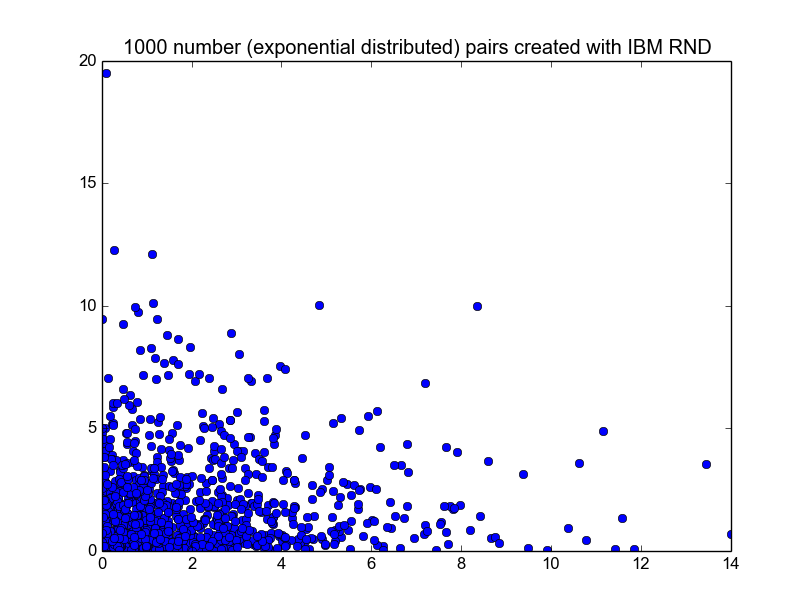
\includegraphics[width=0.8\textwidth]{exponential.png}
            \caption{Exponential distribution function}
            \label{fig:exponential}
        \end{figure}
    \FloatBarrier
    \item See code in \autoref{test} and \autoref{fig:histogram}.
        \begin{figure}[h!]
            \centering
            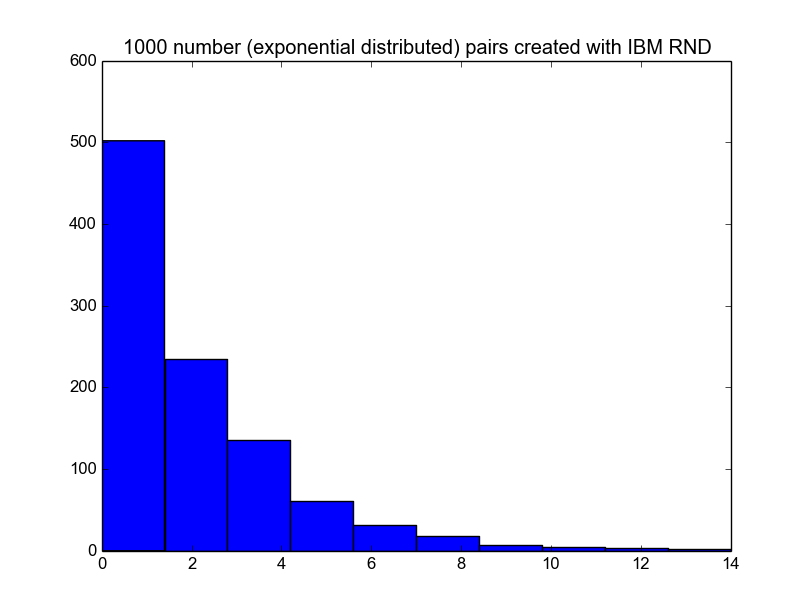
\includegraphics[width=0.8\textwidth]{histogram.png}
            \caption{Histogram of exponential distribution function}
            \label{fig:histogram}
        \end{figure}
    \FloatBarrier
    \item See code in \autoref{test} and \autoref{fig:exponential}.

\end{enumerate}
    \appendix
    \section{Code}
    \label{test}
        {\footnotesize\inputminted{python}{o3.py}}
%TODO More discussion?

% =================================== REFERENCES ===================================

%\clearpage
% \bibliographystyle{apalike}
% \bibliography{report}

\end{document}
